\documentclass[12pt]{article}
\usepackage[utf8]{inputenc}
\usepackage{graphicx}
\renewcommand{\figurename}{Ábra.}

\begin{document}


\section{Bevezetés}

Lorem Ipsum...

\section{Alapok}

\subsection{Neurális hálók}

A neurális hálók biológiai indíttatású programok, amelyek a biológiai neurális hálózat néhány hasznos tulajdonságát modellezik.

\subsubsection{Alapvető felépítése}

A neurális hálók mindössze bonyolult, sok paraméteres, többdimenziós függvények, amelyek egy $n$ dimenziós inputhoz $k$ dimenziós outputot határoznak meg.

Például egy emberhez, pontosabban annak adataihoz hozzárendelnek egy betegséget olyan módon, hogy a négy output közül az veszi fel az $1$ értéket amely betegség a függvény “válasza”, az összes többi (betegséghez tartozó) output pedig $0$. A hálózat tehát meg tudja becsülni, hogy az illető milyen betegségben szenved.

\begin{figure}[h!]
  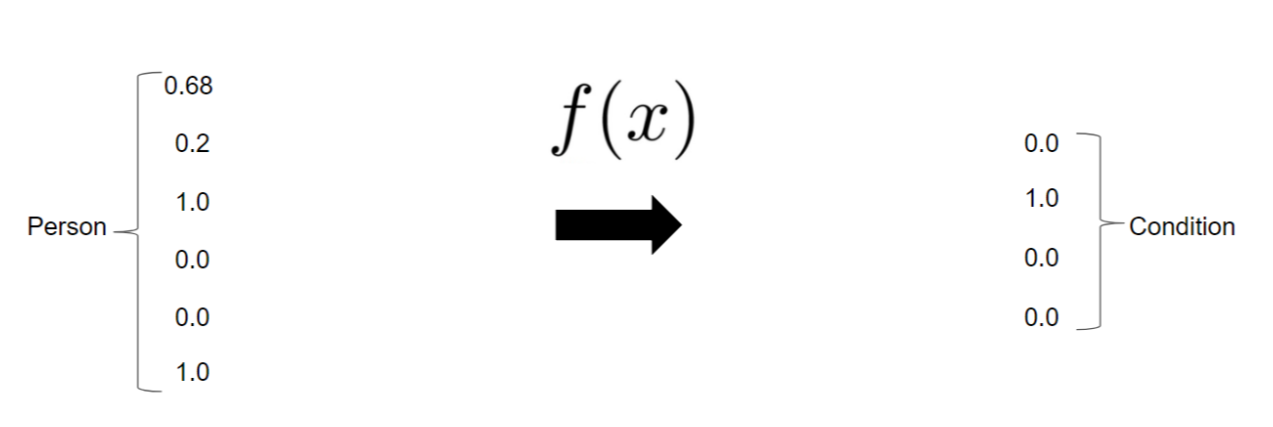
\includegraphics[width=\linewidth]{fgv.png}
  \caption{Általános nézet}
\end{figure}

Ez így elég egyszerűen hangzik, mivel még nem tárgyaltunk arról, hogy ez a függvény hogyan működik, és honnan tud néhány adatból betegségre vonatkozó következtetéseket levonni. A kérdés tehát, hogy hogyan határozzuk meg ezt a függvényt. Legyen a függvény egy neurális háló:

\begin{figure}[h!]
  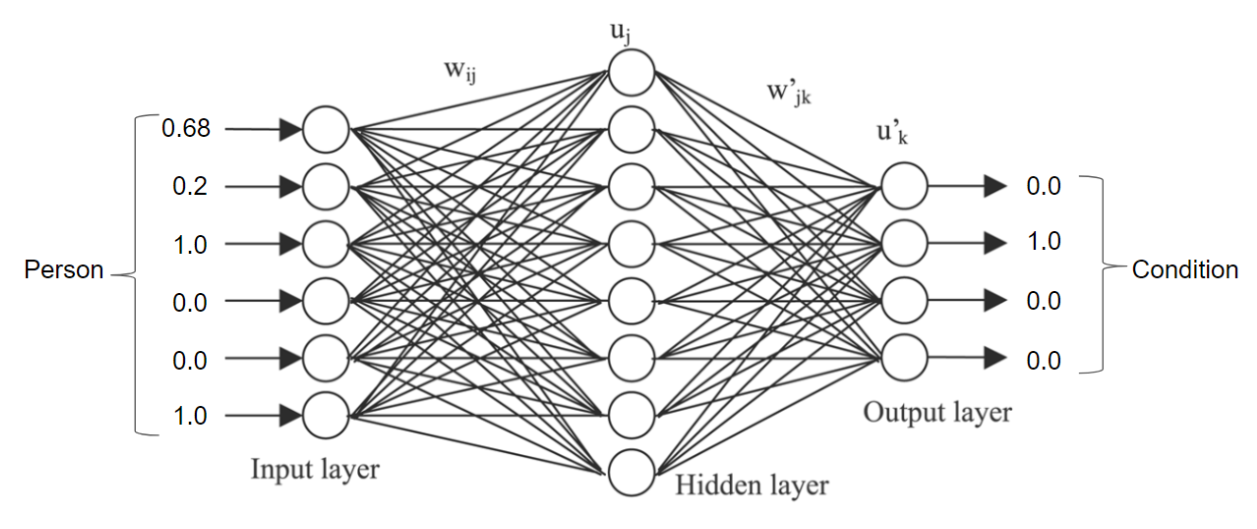
\includegraphics[width=\linewidth]{fgv_network.png}
  \caption{Konkrét neurális háló}
\end{figure}


A neurális háló tulajdonképpen egy súlyozott gráf, melynek n darab csúcsa a bemeneteket reprezentálja, k darab csúcsa pedig a kimeneteket. Az n és k csúcsok halmazát rendre input és output layernek (rétegnek) nevezzük, azonban a maradék csúcsok több kisebb halmazra bonthatóak, az úgynevezett hidden (rejtett) rétegekre. 

Egy egyszerű neurális háló tehát L darab layerből áll, melyek közül az input és output layerek speciális funkciót látnak el. A rétegeknek van egy rögzített sorrendje, amely egy neurális hálónak fix tulajdonsága, sosem változik meg. Sorrendben az első réteg az input layer, amit néhány rejtett réteg követ, majd egy output layer zárja a listát.

Minden réteget neuronok egy halmaza alkot. Ezek a gráf csúcsai. Az élek kizárólag a szomszédos layerek neuronjai között futhatnak. A gráf összes éléhez tartozik továbbá egy-egy valós számértékű súly.

A neuronoknak van egy úgynevezett aktivációs értékük, amely minden pillanatban az az érték, amelyet utoljára - manuálisan vagy automatikusan - beállítottunk neki. Egy neuron aktivációs értéket úgy határozzuk meg, hogy vesszük a neuron rétegét megelőző layer azon neuronjait, amelyekkel össze van kötve, majd vesszük ezeknek a lineáris kombinációját a hozzájuk tartozó élek súlyaival. Ehhez még hozzáadunk egy bias értéket, amely magához a vizsgált neuronhoz tartozik és szintén egy 0 és 1 közé eső skalár.
Ezután még az így kapott összegre alkalmazunk egy úgynevezett aktivációs függvényt, amely ugyancsak a neuronhoz tartozik (bár általában egy rétegben minden ez neuronra azonos).

\begin{figure}[h!]
  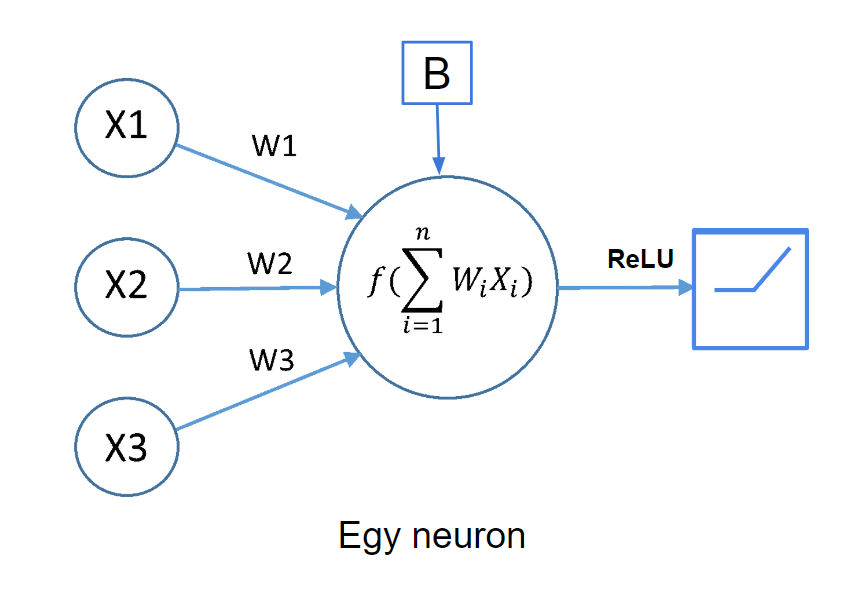
\includegraphics[width=\linewidth]{neuron.png}
  \caption{Általános nézet}
\end{figure}

Az aktivációs függvény rendeltetése, hogy a lineáris kombináció és a bias hozzáadása után keletkezett - várhatóan 1-nél nagyobb - számot visszaskálázzuk a [0-1] intervallumba.
Többféle aktivációs függvény is használhatunk. Gyakoriak:

\subsection{Konvolúciós hálók}

Lorem ipsum dolor sit amet, consectetur adipiscing elit. Fusce at risus quis nibh dignissim venenatis at id lacus. Aenean cursus erat quis magna tempus, sed ultricies est dictum. Donec sed nisl in ante vestibulum hendrerit a id velit. Phasellus vel erat elit. Morbi eu lobortis sem. Pellentesque at nunc et nibh fringilla mattis eu a diam. Cras mollis convallis vestibulum. Donec at mattis est. Duis cursus enim lorem, eu lobortis ante luctus id. Nullam pellentesque convallis quam. Vestibulum laoreet, dolor sed finibus pulvinar, ante felis convallis lorem, quis pulvinar orci ante at ipsum. Etiam facilisis tincidunt tincidunt. Nunc ipsum purus, egestas eu imperdiet vitae, posuere ut odio. Curabitur consectetur ante quis erat venenatis, eget consectetur mauris viverra.

\subsection{Autoencoderek}

Lorem ipsum dolor sit amet, consectetur adipiscing elit. Fusce at risus quis nibh dignissim venenatis at id lacus. Aenean cursus erat quis magna tempus, sed ultricies est dictum. Donec sed nisl in ante vestibulum hendrerit a id velit. Phasellus vel erat elit. Morbi eu lobortis sem. Pellentesque at nunc et nibh fringilla mattis eu a diam. Cras mollis convallis vestibulum. Donec at mattis est. Duis cursus enim lorem, eu lobortis ante luctus id. Nullam pellentesque convallis quam. Vestibulum laoreet, dolor sed finibus pulvinar, ante felis convallis lorem, quis pulvinar orci ante at ipsum. Etiam facilisis tincidunt tincidunt. Nunc ipsum purus, egestas eu imperdiet vitae, posuere ut odio. Curabitur consectetur ante quis erat venenatis, eget consectetur mauris viverra.

\subsection{Generatív modellezés}

Lorem ipsum dolor sit amet, consectetur adipiscing elit. Fusce at risus quis nibh dignissim venenatis at id lacus. Aenean cursus erat quis magna tempus, sed ultricies est dictum. Donec sed nisl in ante vestibulum hendrerit a id velit. Phasellus vel erat elit. Morbi eu lobortis sem. Pellentesque at nunc et nibh fringilla mattis eu a diam. Cras mollis convallis vestibulum. Donec at mattis est. Duis cursus enim lorem, eu lobortis ante luctus id. Nullam pellentesque convallis quam. Vestibulum laoreet, dolor sed finibus pulvinar, ante felis convallis lorem, quis pulvinar orci ante at ipsum. Etiam facilisis tincidunt tincidunt. Nunc ipsum purus, egestas eu imperdiet vitae, posuere ut odio. Curabitur consectetur ante quis erat venenatis, eget consectetur mauris viverra.

\subsection{Variational autoencoderek (VAE)}

Lorem ipsum dolor sit amet, consectetur adipiscing elit. Fusce at risus quis nibh dignissim venenatis at id lacus. Aenean cursus erat quis magna tempus, sed ultricies est dictum. Donec sed nisl in ante vestibulum hendrerit a id velit. Phasellus vel erat elit. Morbi eu lobortis sem. Pellentesque at nunc et nibh fringilla mattis eu a diam. Cras mollis convallis vestibulum. Donec at mattis est. Duis cursus enim lorem, eu lobortis ante luctus id. Nullam pellentesque convallis quam. Vestibulum laoreet, dolor sed finibus pulvinar, ante felis convallis lorem, quis pulvinar orci ante at ipsum. Etiam facilisis tincidunt tincidunt. Nunc ipsum purus, egestas eu imperdiet vitae, posuere ut odio. Curabitur consectetur ante quis erat venenatis, eget consectetur mauris viverra.

\subsection{Módosított variational autoencoderek ($\beta$VAE)}

Lorem ipsum dolor sit amet, consectetur adipiscing elit. Fusce at risus quis nibh dignissim venenatis at id lacus. Aenean cursus erat quis magna tempus, sed ultricies est dictum. Donec sed nisl in ante vestibulum hendrerit a id velit. Phasellus vel erat elit. Morbi eu lobortis sem. Pellentesque at nunc et nibh fringilla mattis eu a diam. Cras mollis convallis vestibulum. Donec at mattis est. Duis cursus enim lorem, eu lobortis ante luctus id. Nullam pellentesque convallis quam. Vestibulum laoreet, dolor sed finibus pulvinar, ante felis convallis lorem, quis pulvinar orci ante at ipsum. Etiam facilisis tincidunt tincidunt. Nunc ipsum purus, egestas eu imperdiet vitae, posuere ut odio. Curabitur consectetur ante quis erat venenatis, eget consectetur mauris viverra.

\section{Implementáció}

Lorem ipsum dolor sit amet, consectetur adipiscing elit. Fusce at risus quis nibh dignissim venenatis at id lacus. Aenean cursus erat quis magna tempus, sed ultricies est dictum. Donec sed nisl in ante vestibulum hendrerit a id velit. Phasellus vel erat elit. Morbi eu lobortis sem. Pellentesque at nunc et nibh fringilla mattis eu a diam. Cras mollis convallis vestibulum. Donec at mattis est. Duis cursus enim lorem, eu lobortis ante luctus id. Nullam pellentesque convallis quam. Vestibulum laoreet, dolor sed finibus pulvinar, ante felis convallis lorem, quis pulvinar orci ante at ipsum. Etiam facilisis tincidunt tincidunt. Nunc ipsum purus, egestas eu imperdiet vitae, posuere ut odio. Curabitur consectetur ante quis erat venenatis, eget consectetur mauris viverra.

\subsection{Az alkalmazott szoftverarchitektúra ismertetése}

Lorem ipsum dolor sit amet, consectetur adipiscing elit. Fusce at risus quis nibh dignissim venenatis at id lacus. Aenean cursus erat quis magna tempus, sed ultricies est dictum. Donec sed nisl in ante vestibulum hendrerit a id velit. Phasellus vel erat elit. Morbi eu lobortis sem. Pellentesque at nunc et nibh fringilla mattis eu a diam. Cras mollis convallis vestibulum. Donec at mattis est. Duis cursus enim lorem, eu lobortis ante luctus id. Nullam pellentesque convallis quam. Vestibulum laoreet, dolor sed finibus pulvinar, ante felis convallis lorem, quis pulvinar orci ante at ipsum. Etiam facilisis tincidunt tincidunt. Nunc ipsum purus, egestas eu imperdiet vitae, posuere ut odio. Curabitur consectetur ante quis erat venenatis, eget consectetur mauris viverra.

\subsection{Dsprite és Celeba adathalmazok}

Lorem ipsum dolor sit amet, consectetur adipiscing elit. Fusce at risus quis nibh dignissim venenatis at id lacus. Aenean cursus erat quis magna tempus, sed ultricies est dictum. Donec sed nisl in ante vestibulum hendrerit a id velit. Phasellus vel erat elit. Morbi eu lobortis sem. Pellentesque at nunc et nibh fringilla mattis eu a diam. Cras mollis convallis vestibulum. Donec at mattis est. Duis cursus enim lorem, eu lobortis ante luctus id. Nullam pellentesque convallis quam. Vestibulum laoreet, dolor sed finibus pulvinar, ante felis convallis lorem, quis pulvinar orci ante at ipsum. Etiam facilisis tincidunt tincidunt. Nunc ipsum purus, egestas eu imperdiet vitae, posuere ut odio. Curabitur consectetur ante quis erat venenatis, eget consectetur mauris viverra.

\subsection{Látens reprezentációk strukturáltságának számszerűsítése}

Lorem ipsum dolor sit amet, consectetur adipiscing elit. Fusce at risus quis nibh dignissim venenatis at id lacus. Aenean cursus erat quis magna tempus, sed ultricies est dictum. Donec sed nisl in ante vestibulum hendrerit a id velit. Phasellus vel erat elit. Morbi eu lobortis sem. Pellentesque at nunc et nibh fringilla mattis eu a diam. Cras mollis convallis vestibulum. Donec at mattis est. Duis cursus enim lorem, eu lobortis ante luctus id. Nullam pellentesque convallis quam. Vestibulum laoreet, dolor sed finibus pulvinar, ante felis convallis lorem, quis pulvinar orci ante at ipsum. Etiam facilisis tincidunt tincidunt. Nunc ipsum purus, egestas eu imperdiet vitae, posuere ut odio. Curabitur consectetur ante quis erat venenatis, eget consectetur mauris viverra.

\subsection{Vizualizációs eszközök ismertetése}

Lorem ipsum dolor sit amet, consectetur adipiscing elit. Fusce at risus quis nibh dignissim venenatis at id lacus. Aenean cursus erat quis magna tempus, sed ultricies est dictum. Donec sed nisl in ante vestibulum hendrerit a id velit. Phasellus vel erat elit. Morbi eu lobortis sem. Pellentesque at nunc et nibh fringilla mattis eu a diam. Cras mollis convallis vestibulum. Donec at mattis est. Duis cursus enim lorem, eu lobortis ante luctus id. Nullam pellentesque convallis quam. Vestibulum laoreet, dolor sed finibus pulvinar, ante felis convallis lorem, quis pulvinar orci ante at ipsum. Etiam facilisis tincidunt tincidunt. Nunc ipsum purus, egestas eu imperdiet vitae, posuere ut odio. Curabitur consectetur ante quis erat venenatis, eget consectetur mauris viverra.

\subsection{Kísérletek}

Lorem ipsum dolor sit amet, consectetur adipiscing elit. Fusce at risus quis nibh dignissim venenatis at id lacus. Aenean cursus erat quis magna tempus, sed ultricies est dictum. Donec sed nisl in ante vestibulum hendrerit a id velit. Phasellus vel erat elit. Morbi eu lobortis sem. Pellentesque at nunc et nibh fringilla mattis eu a diam. Cras mollis convallis vestibulum. Donec at mattis est. Duis cursus enim lorem, eu lobortis ante luctus id. Nullam pellentesque convallis quam. Vestibulum laoreet, dolor sed finibus pulvinar, ante felis convallis lorem, quis pulvinar orci ante at ipsum. Etiam facilisis tincidunt tincidunt. Nunc ipsum purus, egestas eu imperdiet vitae, posuere ut odio. Curabitur consectetur ante quis erat venenatis, eget consectetur mauris viverra.

\subsubsection{Tanulási idő hatása}

Lorem ipsum dolor sit amet, consectetur adipiscing elit. Fusce at risus quis nibh dignissim venenatis at id lacus. Aenean cursus erat quis magna tempus, sed ultricies est dictum. Donec sed nisl in ante vestibulum hendrerit a id velit. Phasellus vel erat elit. Morbi eu lobortis sem. Pellentesque at nunc et nibh fringilla mattis eu a diam. Cras mollis convallis vestibulum. Donec at mattis est. Duis cursus enim lorem, eu lobortis ante luctus id. Nullam pellentesque convallis quam. Vestibulum laoreet, dolor sed finibus pulvinar, ante felis convallis lorem, quis pulvinar orci ante at ipsum. Etiam facilisis tincidunt tincidunt. Nunc ipsum purus, egestas eu imperdiet vitae, posuere ut odio. Curabitur consectetur ante quis erat venenatis, eget consectetur mauris viverra.

\subsubsection{$\beta$ hiperparaméter hatása}

Lorem ipsum dolor sit amet, consectetur adipiscing elit. Fusce at risus quis nibh dignissim venenatis at id lacus. Aenean cursus erat quis magna tempus, sed ultricies est dictum. Donec sed nisl in ante vestibulum hendrerit a id velit. Phasellus vel erat elit. Morbi eu lobortis sem. Pellentesque at nunc et nibh fringilla mattis eu a diam. Cras mollis convallis vestibulum. Donec at mattis est. Duis cursus enim lorem, eu lobortis ante luctus id. Nullam pellentesque convallis quam. Vestibulum laoreet, dolor sed finibus pulvinar, ante felis convallis lorem, quis pulvinar orci ante at ipsum. Etiam facilisis tincidunt tincidunt. Nunc ipsum purus, egestas eu imperdiet vitae, posuere ut odio. Curabitur consectetur ante quis erat venenatis, eget consectetur mauris viverra.

\subsubsection{Konvolúciós architektúra hatása}

\end{document}
